\chapter{Project Choice}
The first step in my EPQ journey was to fill out the personal Audit form over the summer which helped me to identify my interests and explore some ideas that could link to project ideas
\section{Personal Audit and Reflection}

\begin{enumerate}
    \item \textbf{What do you do in your spare time?} Engage with my hobbies such as computer science and technical theatre, play sports (my main being rugby), practise my instrument (tuba), and play games with friends and family online.

    \item \textbf{What do you watch on YouTube? Why?} I usually watch informative content focused around computer science to further my skills.

    \item \textbf{Which Instagram accounts do you follow? Why?} I primarily follow friends and family to share life moments with them. I also follow a few niche influencers within my hobbies to participate with their communities.

    \item \textbf{What are your favourite things to watch on Netflix/TV/iPlayer/Prime?} When watching content purely for entertainment, I enjoy science fiction shows such as Star Wars and the Marvel franchise.

    % \item \textbf{Which real or imaginary character do you identify with most? Why?} [No answer provided.]

    \item \textbf{What is your bucket list of things to complete by the time you are 25?} While I haven't made myself a bucket list of activities to complete, I have set myself goals for what I want to achieve. These include exploring the world, finding myself a career I will love, and spending time with family.

    \item \textbf{Any good books you have read recently? Is there a genre you like?} With exams just off the horizon, most of my current reading has been purely for academic gain. Unfortunately, with all my digital hobbies, reading literature has become less frequent for me, but I hope to reverse this trend throughout my time in Sixth Form.

    \item \textbf{How do you feel about sport?} Throughout my life I have always been keen on playing sport. Preferring team sports for their additional community aspect, I have played cricket and rugby for both school and club, in addition to many others (such as football and hockey) more leisurely. Approaching adulthood, my favourite sport is rugby for the physical and social benefits it provides.

    \item \textbf{What sort of music do you like?} Having worked in audio storytelling (through my technical theatre work focused on audio mixing and film), I have been exposed to such a wide range of genres that I really don't have a strong preference. Just play a song out loud, and I'm sure to love it.

    \item \textbf{Favourite song? Best lyrics? Best album cover? Best music video?} Although a mainstream song, I am a fan of \textit{Believer} by Imagine Dragons. That song was playing during my life's happiest moments and continues to always inspire me.

    \item \textbf{What would you go on a protest march in support of?} I believe that acceptance for all is the fundamental basis for equality and would support a movement pushing for this fundamental goal.

    \item \textbf{Are there any political events currently that have grabbed your attention?} Political history of nations and technological developments underpinning modern militaries are hugely fascinating to me. As such, I have been closely following the events unfolding in the Middle East, the Russian/Ukrainian border, and the China–Taiwan Strait. Closer to home, I also keenly follow British politics and petitioned policies.

    \item \textbf{How do you feel about artistic skills?} While I appreciate the skills many people have, I personally do not possess these and am much more comfortable working within a digital domain.

    \item \textbf{How do you feel about crafts and creating things?} Whilst I enjoy learning from and using products created by skilled craftspeople, I lack the fine skills to produce these items myself. Instead, I choose to focus my skills around CAD/CAM (computer-aided design/manufacture), which allows me to bring my digital creations to the physical world.

    \item \textbf{How do you feel about working with digital media?} Integrating with all of my hobbies, digital mediums of work are my most interacted with. Mediums include film, photography, audio recordings, 3D modelling, etc.

    \item \textbf{What item of clothing you possess best represents you? What is your favourite outfit?} Practising function over form, I don't think a pair of jeans and a t-shirt can be beaten. Though I do enjoy dressing up in formal wear for business events.

    \item \textbf{If you could learn anything what would that be?} I would want to learn the raw biological skills that underpin the human thought process. This knowledge would help link with my computer science passions to further revolutionise the development of AI to better the world.

    \item \textbf{What subjects are you studying at A level?} I will be studying: Computer Science, Physics, Maths, and Further Maths.

    \item \textbf{Is there anything you wish you could have taken at A level but are not?} Not especially, I am fortunate to have achieved the grades required for my chosen subject combination.

    \item \textbf{How do you relax?} I most enjoy relaxing with friends and family; playing sports, having fun and spending quality time together.
\end{enumerate}


\section{Project Ideas}
I was then fortunate to have a day focused on the EP my EPQ coordinator, where i learnt more about the skills i would need to develop and the process of completing an EPQ. This day also allowed me to explore some project ideas that could be suitable for my EPQ.
\begin{figure}[H]
    \centering
    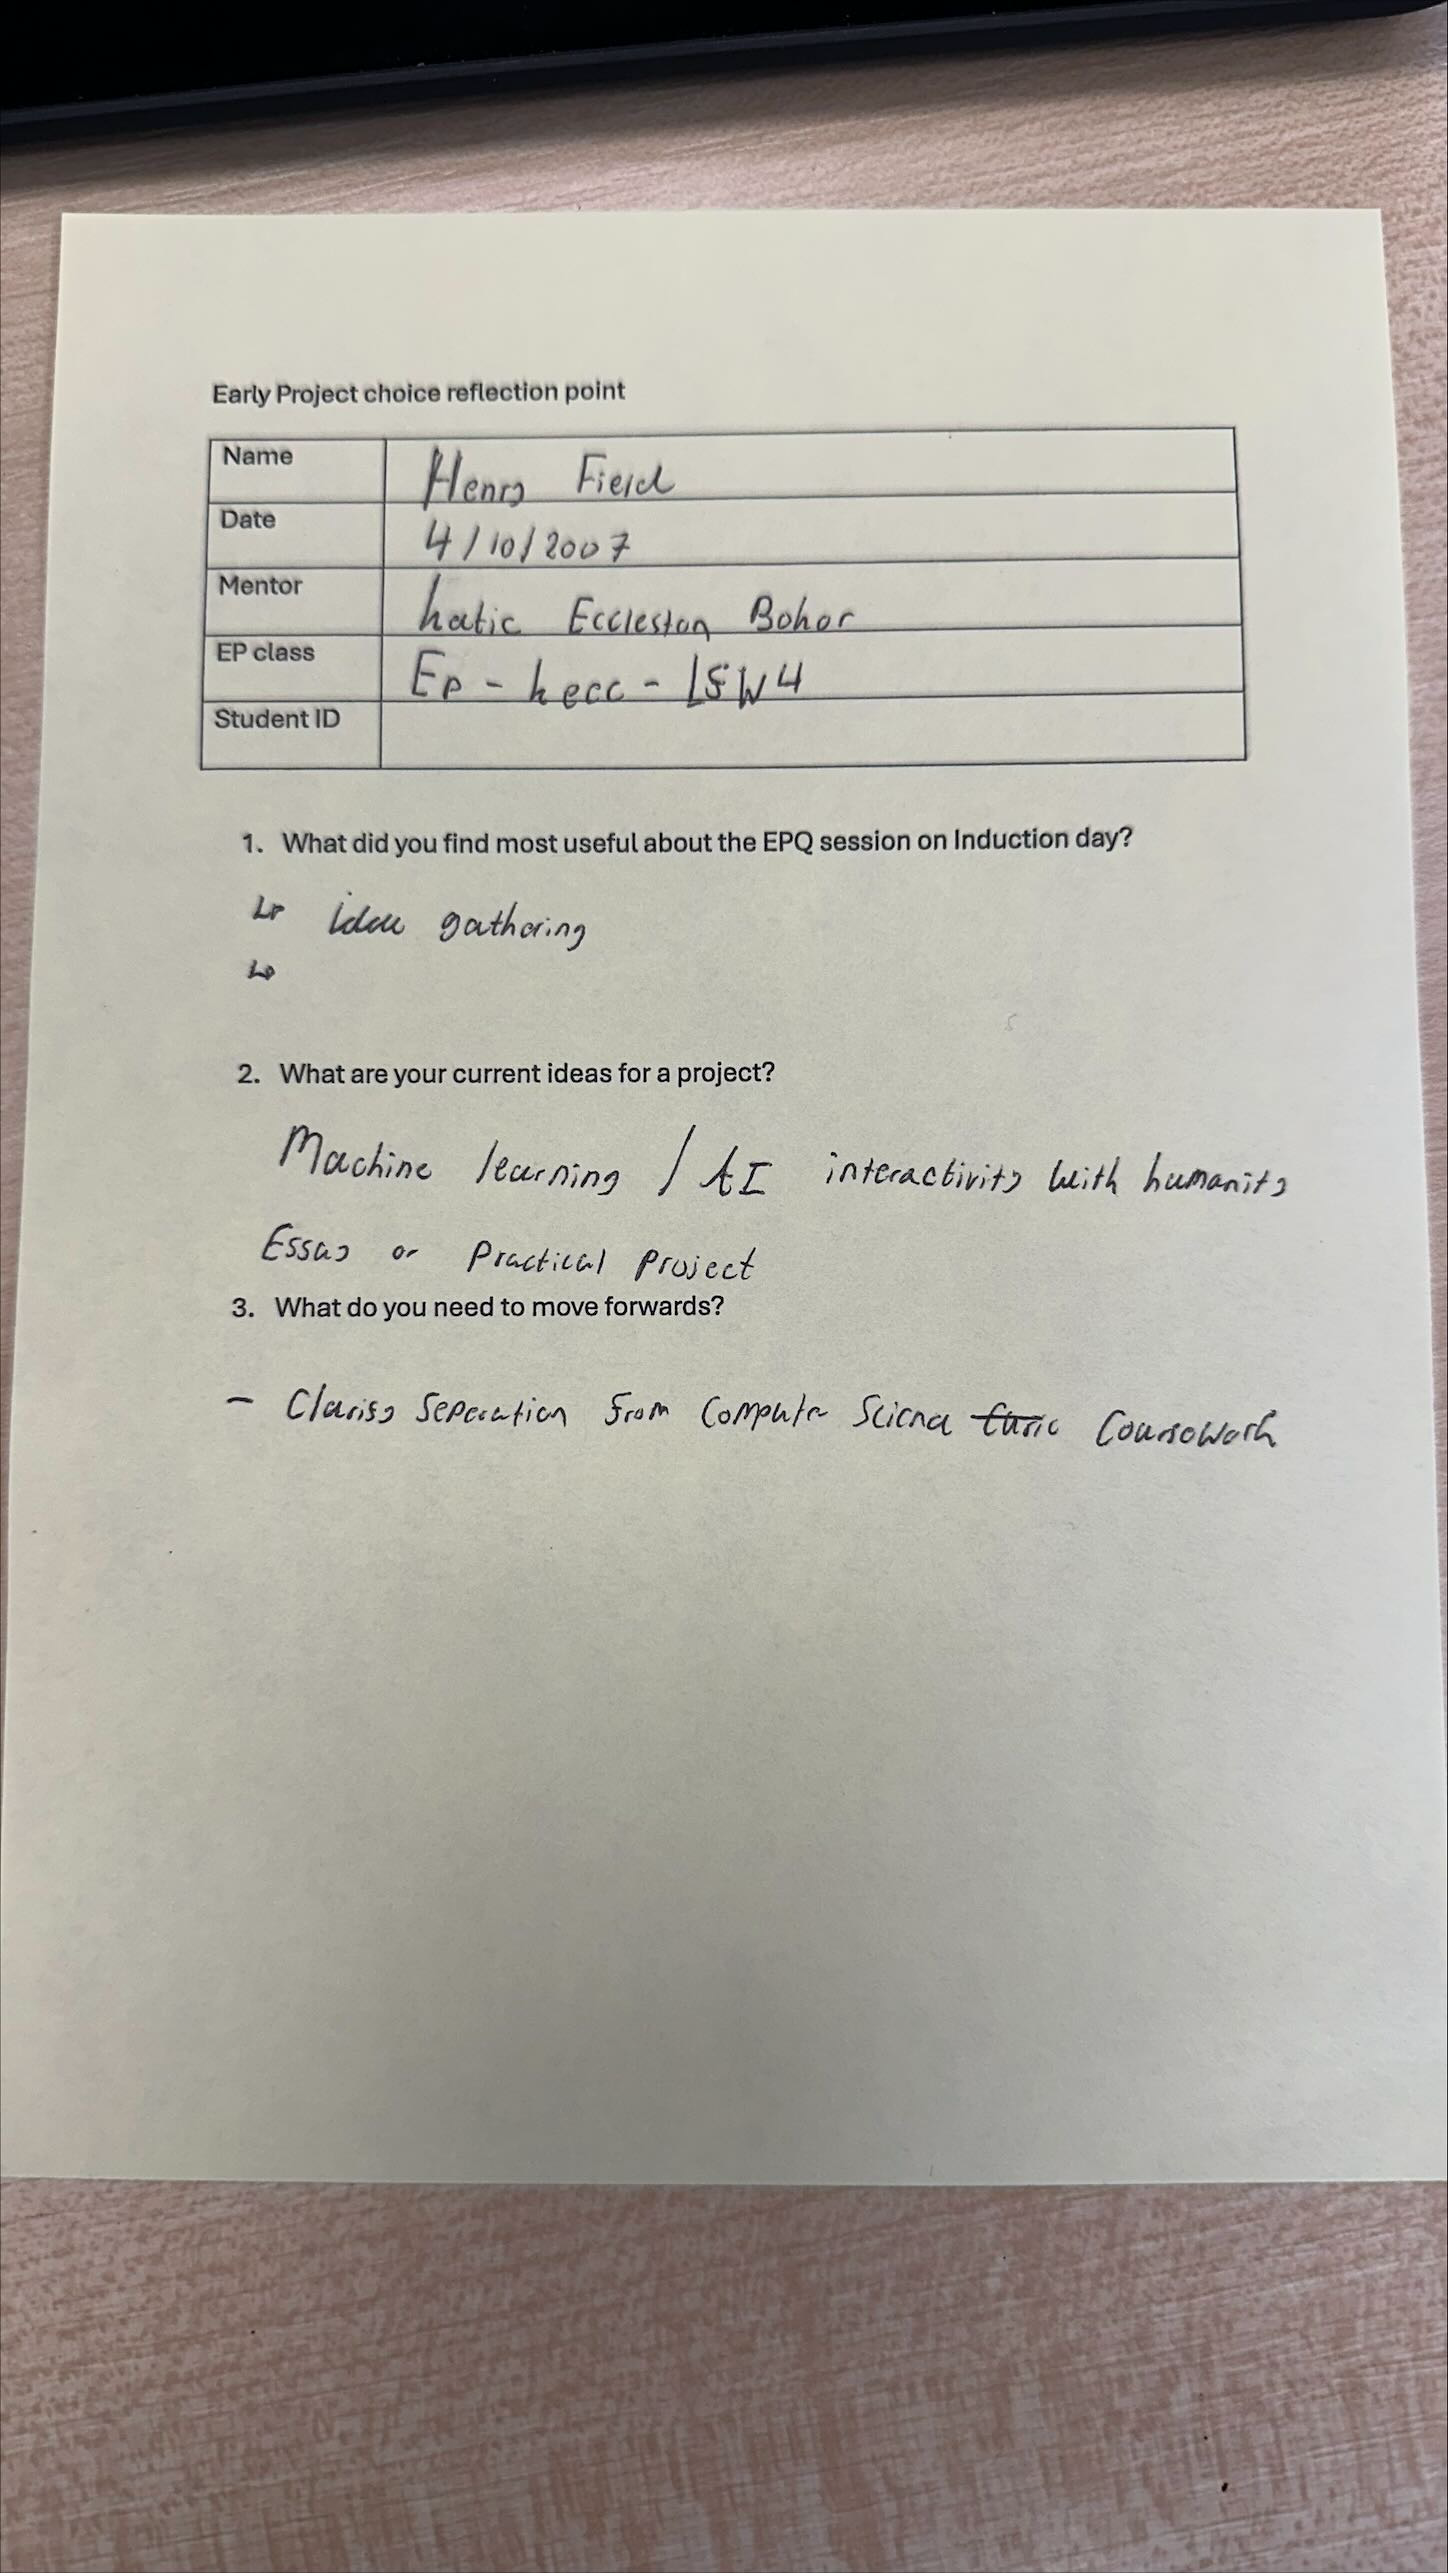
\includegraphics[width=0.3\textwidth]{ProjectChoice/Media/EarlyProjectChoiceReflection.png}
    \caption{Early Project Choice Reflection}
    \label{fig:EarlyProjectChoiceReflection}
\end{figure}
Next I spent some time reflecting on the ideas i had and how they could be developed into a project. To help me map out my thoughts I produced a Mindmap of the various ideas i could explore
\begin{figure}[H]
    \centering
    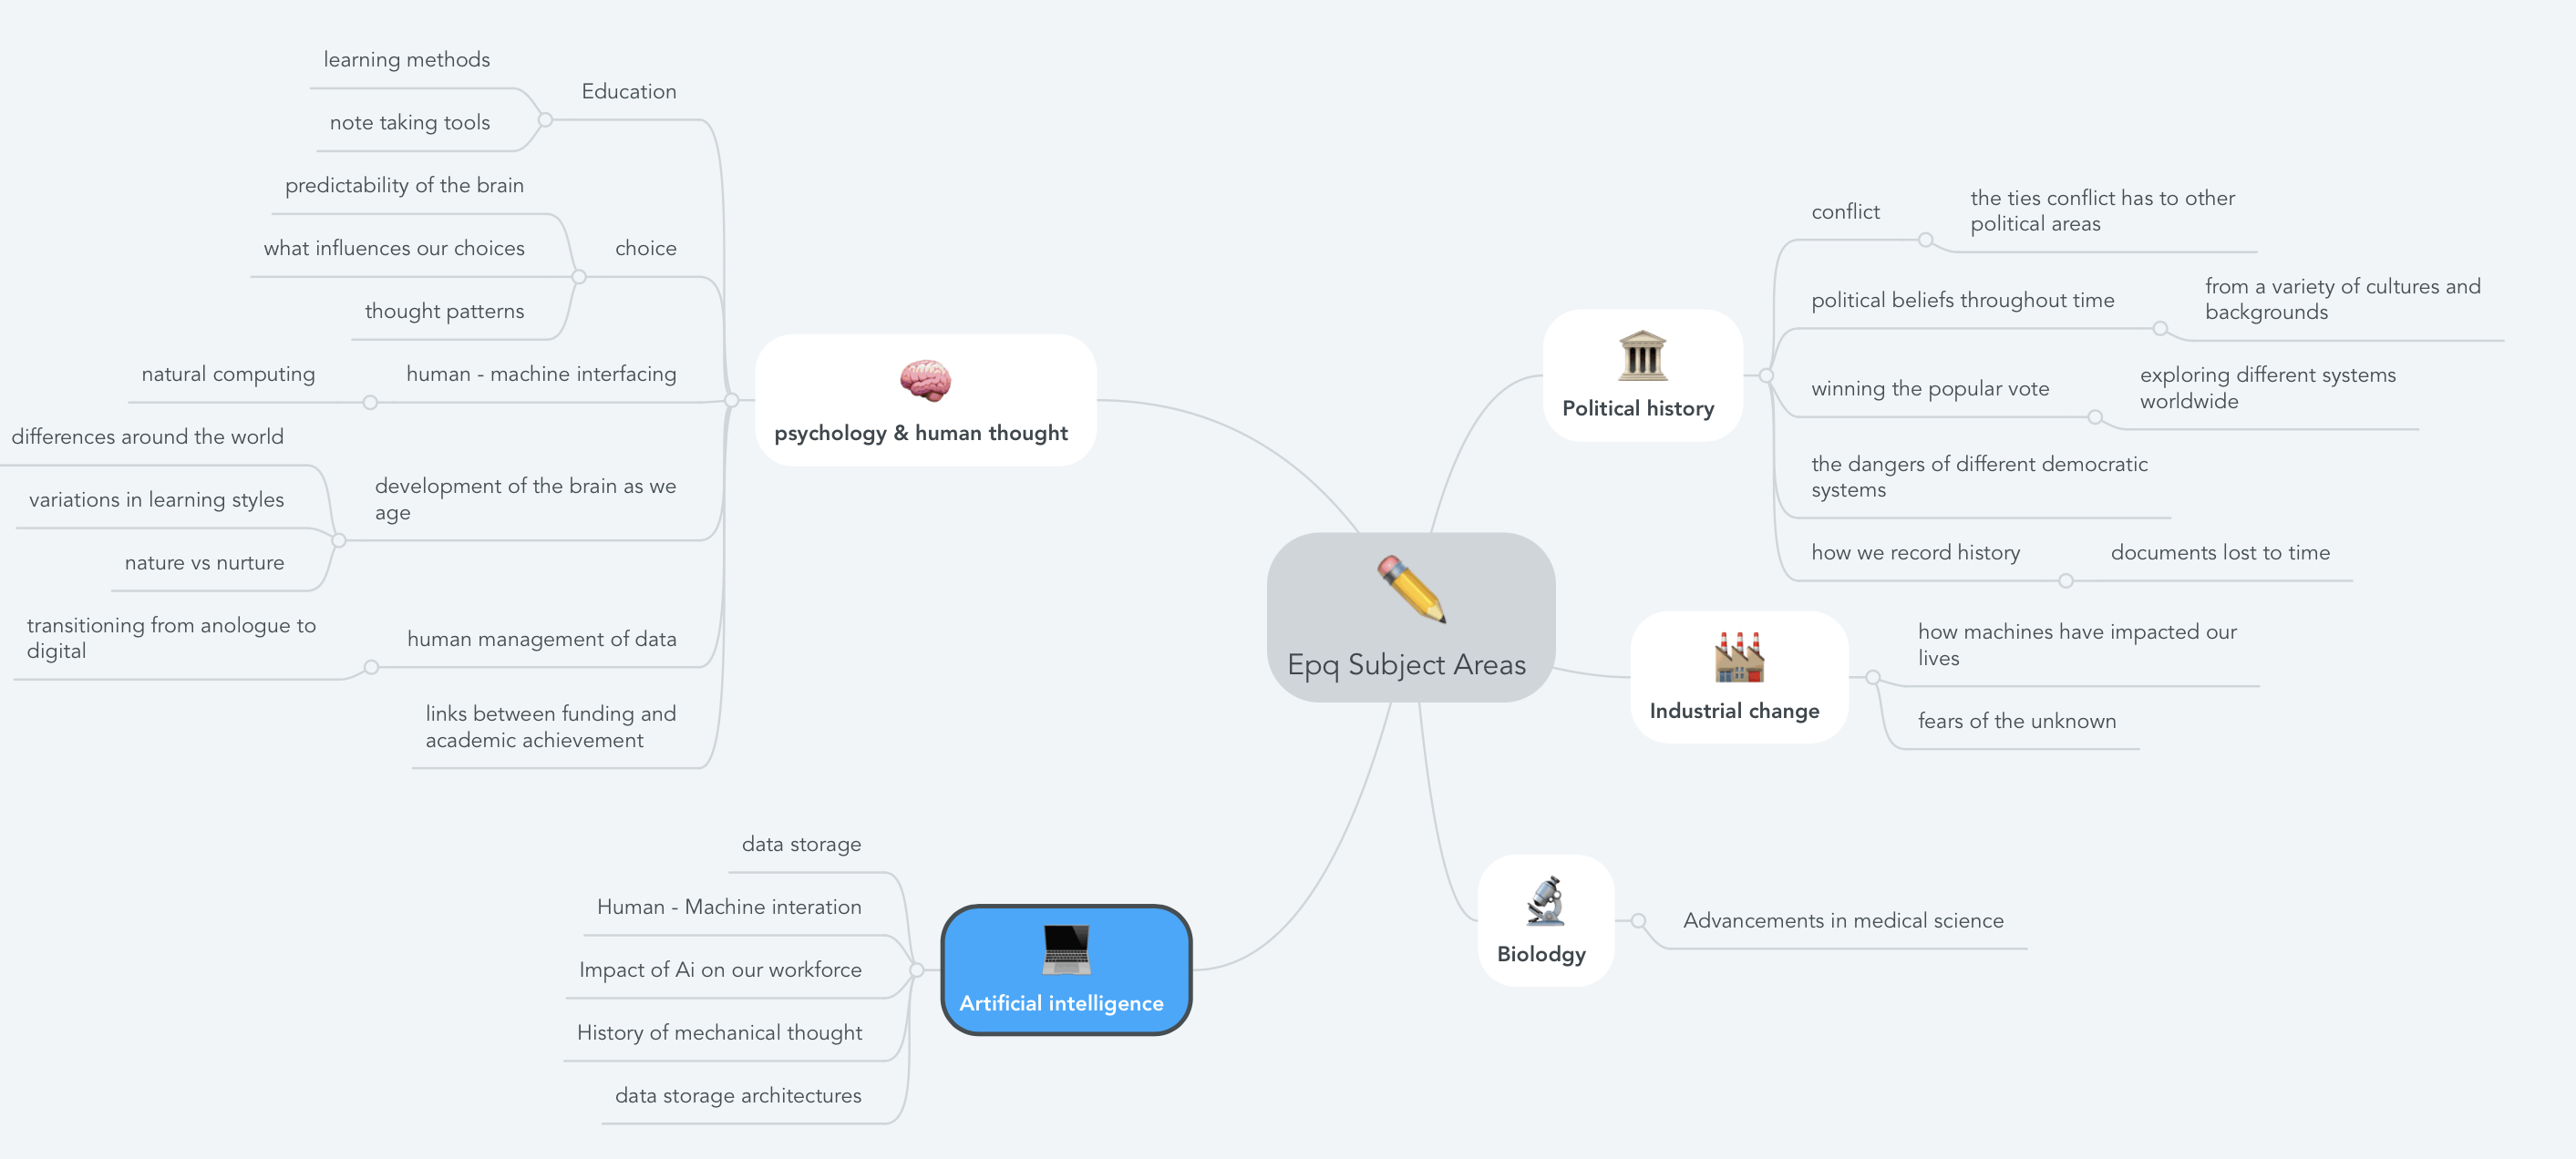
\includegraphics[width=0.9\textwidth]{ProjectChoice/Media/Mindmap.png}
    \caption{Mindmap of my ideas}
    \label{fig:EarlyProjectChoiceMindmap}
\end{figure}

Finally (after much careful deliberation) i was able to narrow down my ideas and select a project to pursue.
\section{Final Project Selection}
Having spent the last few weeks researching various topics as outlined in my mind map. I have now decided on my EPQ project.

Considering the topics I researched and identified in my mind map, I want to integrate Digital workflows, , human learning, web development and tools useful for everyday life. Therefore I have decided to investigate building a software Note storage system designed for students to enable them to quickly search their notes and organise their educational and personal lives. While similar tools do exist (and I have compared in my research section) I haven't found any which fit my (and others) needs and don’t have huge sacrifices that must be made.

While my list of requirements is ever changing (and will be outlined throughout my diary as they progress) these are my base musts for my project to be successful:
\begin{itemize}
	\item Ability to view and edit notes from anywhere, and on any device (laptop, phone, pc and even a smart fridge)
	\item Ability to quickly find any notes anywhere and make logical links between notes for exploration
	\item Robust collaboration tools for working with peers and sharing information
	\item Ability to store text, images and even handwriting within notes
	\item Simple setup and file management  
\end{itemize}
My end goal is to produce software I can use for all my studies and for collating all of my EPQ notes (as OneNote doesn’t quite cover my needs - hence the need for improvement in the space) 

Whilst choosing my project I did have some concerns regarding overlap with the A Level computer science course I am taking. I therefore communicated with both my Computer science teacher and Course mentor to gather their opinions. After an in-person conversation we decided that whilst there are similarities to an extent between a potential computer science NEA (which doesn't start until Y13) and my project,  my project would be distinct enough providing I document all of my learnings to great depth and leaned towards the impact research on human learning has had than  towards the direction of my final software artifact

From past experience of both projects I have worked on and have watched from afar that 'scope creep' can (more often than not) have a huge negative impact on the end produced result. To mitigate this in addition to the core values mentioned above I am going to keep an updating document linked to my timeline which included features I know that can be feasibly added in and some stretch goals that I will add only if time permits. I am hopeful that this management and planning will result in me achieving my goals and possibly even developing my project into a tool I can carry with my to university and beyond, but all in good time.

Below is a table of my current project requirements and how I plan to tackle them. This will be updated as I progress through my project and will be used to help me keep track of my progress and ensure I am on track to meet my goals.


\begin{tabularx}{\textwidth}{
    >{\raggedright\arraybackslash}l 
    >{\raggedright\arraybackslash}X 
    >{\raggedright\arraybackslash}X
}
\toprule
\textbf{Task/Feature} & \textbf{Description} & \textbf{Action Plan} \\
\midrule

\rowcolor{gray!10}
\multicolumn{3}{l}{\textbf{High Priority \& High Impact (Do First)}} \\

Core software development & Building the foundational system for note-taking, organization, and accessibility. & Begin development with a focus on core functionalities. \\

Cross-device accessibility & Ensuring the system works on multiple devices (laptop, phone, smart fridge, etc.). & Research frameworks that support multi-platform use. \\

Fast search \& logical links & Implementing a system to quickly find notes and establish relationships between them. & Prioritize efficient indexing and search algorithms. \\

Human learning research integration & Designing the tool based on effective study methods. & Document findings and integrate best practices. \\

\rowcolor{gray!10}
\multicolumn{3}{l}{\textbf{High Priority \& Low Impact (Plan for Later)}} \\

Collaboration tools & Features for peer sharing and real-time collaboration. & Plan architecture but implement later. \\

Handwriting \& multimedia support & Adding handwritten note storage and image support. & Research existing libraries for ease of integration. \\

File management & Ensuring an intuitive and simple organization system. & Define structure before implementation. \\

\rowcolor{gray!10}
\multicolumn{3}{l}{\textbf{Low Priority \& High Impact (Delegate/Streamline)}} \\

Stretch goals \& enhancements & Additional features that improve usability but aren’t core. & Maintain an evolving feature backlog. \\

Advanced AI search suggestions & Smart recommendations for note retrieval. & Implement if time allows. \\

\rowcolor{gray!10}
\multicolumn{3}{l}{\textbf{Low Priority \& Low Impact (Eliminate or Delay)}} \\

Extensive UI customization & Custom themes, animations, or unnecessary aesthetics. & Keep UI minimal for now. \\

Full-scale competitor comparison & While helpful, extensive comparisons may not be crucial. & Summarize findings instead of deep-dive analysis. \\

\bottomrule
\end{tabularx}
\label{projectchoice:prioritymatrix}
